\section{Analyst in control}

Throughout our study we observed that analysts are constantly annotating new data, restructuring existing annotations, archiving irrelevant data, and examining data in visualization. This is an extension compared to many other visualization tools, with which users are faced with pre-populated data and tasked with creating visual mappings to identify hidden patterns behind the data. In Intelligence Analysis and many other information analysis tasks, analysts frequently create and re-recreate data models to serve their analysis as their hypothesis evolves.

Data modeling is often seen as a precondition to perform any visual analysis. Data modeling transforms raw data to structured entities that are readable and processable to software. The focus of Visual Analytics has been largely put on combining automated modeling with interactive visualizations to facilitate reasoning \citep{Keim2010}, emphasizing the role of human in the loop of visualization and insight generation. In practice, however, we find that data modeling is an iterative process that is intermingled with visual analysis. New insights inspires analysts to re-model data either in a different scope (horizontally) or in a different level of detail (vertically). 

Horizontally, analysts annotate different parts of the data. For example, an intelligence project typically includes data that consists of a series of \textit{critical events}. Analysis of the data though can focus on some of the events. Analysts decide which events to look into first. As they come up with new hypotheses or need more data to validate his hypothesis, they may continue annotating and visualizing other events.

Vertically, analysts annotate data to the level of detail they prefer at the moment of their analysis. The same piece of a document can be annotated in different ways according to the analyst's need. For example, when the analysts are in the early phase of the investigation and want to get an overview of all events, they can annotate an event with time, place, and a brief summary. As they get more interested in a specific event, they can add the people that were involved and tools/resources that were used in the event. If the event becomes critical and needs to be compared with other events to find patterns, analysts might annotate the step-by-step process how people did it in the event. In contrast, if an event becomes irrelevant to the hypothesis, the analysts may remove its details or the event altogether to avoid distraction. 

We use annotation to allow analysts to create and modify their data of interest. This complements the popular approach which employs 
automated modeling such as natural language processing (NLP) techniques to extract and
model entities \citep{Bier2010, Stasko2008}. While algorithms for named
entity recognition have improved significantly, developers of the
entity-based systems \citep{Gorg2014} admitted that the
accuracy of automatic entity extraction is not sufficient to support
human analysis. This is especially true when the tasks are exploratory in nature, where the questions are ill-defined and no training data is available \citep{thomas2005illuminating}. Besides, relationships identified by algorithms are
limited to the co-occurrence of entities in the same document, whereas
identifying meaningful relationships \emph{implicit} in documents that
are of more importance to analysts is not possible. And perhaps the most
problematic is the fact that the NLP treats all pieces of information
equally with no regard to the problem analysts have at hand. 

We posit
that information analysis is a progressive process, wherein analysts
place a varying priority on evidence depending on how they frame the
problem \citep{Heuer1999}. Annotation allows for user
control in the process, allows integrated source data objects to be identified,
and avoids the problems associated with automatic identification of
disaggregated people, locations, and times \citep{Bier2008}. Analysts can
decide their own information of interest and granularity that best suits
their ad-hoc analytic needs. The guide to visually exploring data ``Overview first, zoom and filter, then details-on-demand'', as proposed by \cite{shneiderman2003eyes} describes how data should be presented on screen. We suggest extending the guide to be ``Overview first, model data, analyze, zoom and filter, re-model, then details on demand''.

\section{Collaboration, structured technique, and the role of computing tools}

Collaboration is, in essence, the development of \textit{content} common ground and \textit{process} common ground within a team \citep{Convertino2009}. Content common ground encompasses ``I know that you know that I know \textit{what}''. It is the result of information sharing. Process common ground encompasses ``I know that you know that I know \textit{how}''. This is the shared understanding across team members of the procedures, rules, and manner in which collaboration will occur. Process common ground helps teams achieve high awareness and result in content common ground.

Process common ground can be achieved with ad-hoc team discussion and negotiation, or agreement on a predefined set of procedures. Structured technique is such a predefined set of procedures, rules, and manner in information analysis. Structured technique breaks down information analysis into a defined process of reasoning, and define a set of procedures teammates agree upon \textit{before} they start to collaborate on work. With all analysts understanding the structured technique, it provides teams with a base process common ground. Following the structured techniques, each team member has their role and task. By implementing the technique, individuals focus on their own piece of work, while understanding what and why teammates are working on, without constantly re-coordinating and re-aligning team intentions and individual behaviors. Structured technique has little dependency on the team attributes or individual experience, and thus can be applied to various teams with relative ease. In that sense, It is a methodology of common ground development that can be abstracted and generalized to collaboration between other teams, to enable effective teamwork. 

Structured technique emphasizes the externalization of reasoning and preserve the process that leads to the conclusion. Human mind is often blamed for its stateless memory--people keep updated with the current thinking, but lose track of the last idea even seconds ago. Information analysis typically takes an extended period of time, and the final conclusion may differ completely from the original hypothesis. The situation becomes even worse in collaborative work. People fail to recall arguments or evidence from teammates. Structured techniques help organize information in a structured manner. For example, our tool requires analysts to put facts and relationships in a structured form. These representations can easily be shared across teammates. With real time sharing, every creation or modification of externalization is streamed to teammates as partner's action along the course, contributing to the development of team awareness. Structured technique preserves the path of reasoning, including the proposal of a hypothesis, evidence favoring or against the hypothesis, and development of the hypothesis. Such information provides references to team collaboration, anchors over which teams can discuss and improve.

Structured techniques are yet tedious to implement manually. It requires a lot of effort to externalize information and keep it organized. This is where computing tools come in. Computers are efficient at keeping consistent data structures and make cross-referencing data entities straightforward. There are at least four functions computing tools can support: 1) Keeping data input consistent from collaborators. Individuals from different backgrounds and roles could have different input habits and formats. The tool can enforce a format that complies with the structured technique. 2) Visualize information. 3) Share information and team actions properly. 4) Identify opportunities for collaboration.

\begin{figure}
	\centering
	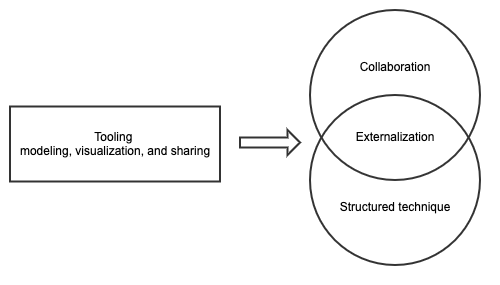
\includegraphics[width=\columnwidth]{06-Discussion/img/theory.png}
	\caption{Structured techniques, collaboration, and tooling}
\end{figure}

